%% Requires compilation with XeLaTeX or LuaLaTeX
\documentclass[10pt,xcolor={table,dvipsnames},t]{beamer}
\usetheme[background=dark]{trigon}
\usepackage{amsmath}
\usepackage{nicefrac}
\usepackage{amssymb}
%\usepackage{enumitem}
\usepackage{braket}
\usepackage{empheq}
\usepackage{color}
\usepackage{keyval}
\usepackage{subcaption}
\usepackage{calrsfs}
\usepackage{hyperref}
\usepackage{eufrak}
\usepackage{transparent}

\captionsetup{font=scriptsize}
\title{Open Quantum System}
\subtitle{
  Lectures: \\ 
  \footnotesize
  \begin{itemize}
      \setlength\itemsep{-0.5em}
    { 
      \transparent{0.4}
    \item[] Last time:
    \item Daniel Manzano, A short introduction to the Lindblad master equation (\textit{all})
    \item Breuer and Petruccione, The Theory of Open Quantum Systems (\textit{ch. 3 - 4.3})
    \item Daniel A. Lidar, Notes on the Theory of Open Quantum Systems (\textit{up to ch. 12})
    }
  \item[] Today:
    \item Breuer and Petruccione, The Theory of Open Quantum Systems (\textit{ch. 3 - 4.3})
    \item Daniel A. Lidar, Notes on the Theory of Open Quantum Systems (\textit{up to ch. 12})
    \item B.Kraus, H.P.Buchler, S. Diehl, A. Kantian, A. Micheli, \& P. Zoller, Preparation of Entangled States by Quantum Markov Processes
    \item Buča, B., Tindall, J. \& Jaksch, D. Non-stationary coherent quantum many-body dynamics through dissipation
    \item Victor V. Albert \& Liang Jiang, Symmetries and conserved quantities in Lindblad master equations
    \item Cameron Booker, Berislav Buča, Dieter Jaksch, Non-stationarity and Dissipative Time Crystals: Spectral Properties and Finite-Size Effects
  \end{itemize}
  \vspace{-1cm}
}
\newcommand{\dt}{\frac{d}{dt}}
\newcommand{\lan}{\mathcal{L}}
\newcommand{\Hint}{H_{\text{int}}}
\newcommand{\outerprod}[2]{\ket{#1}\!\!\bra{#2}}
\newcommand{\tr}[2]{\text{Tr}_{#1}\bigl[#2\bigr]}
\newcommand{\kett}[1]{\vert #1 \rangle\!\rangle}

\setbeamertemplate{footline}{
  \hbox{%
    \begin{beamercolorbox}[wd=.5\paperwidth,ht=2.5ex,dp=1ex,left]{author in head/foot}%
      %\usebeamerfont{author in head/foot}\insertshortauthor~~(\insertshortinstitute)
    \end{beamercolorbox}%
    \begin{beamercolorbox}[wd=.5\paperwidth,ht=2.5ex,dp=1ex,right]{title in head/foot}%
    \end{beamercolorbox}}%
  \vskip0pt%
}

\newlength\mytemplen
\newsavebox\mytempbox
\usepackage{accents}
\newlength{\dhatheight}

\newcommand{\doublehat}[1]{%
    \settoheight{\dhatheight}{\ensuremath{\hat{#1}}}%
    \addtolength{\dhatheight}{-0.15ex}%
    \hat{\vphantom{\rule{1pt}{\dhatheight}}%
    \smash{\hat{#1}}}}

\newcommand\mybluebox{%
    \@ifnextchar[%]
       {\@mybluebox}%
       {\@mybluebox[0pt]}}

\definecolor{myblue}{rgb}{.8, .8, 1}

\def\@mybluebox[#1]{%
    \@ifnextchar[%]
       {\@@mybluebox[#1]}%
       {\@@mybluebox[#1][0pt]}}

\def\@@mybluebox[#1][#2]#3{
    \sbox\mytempbox{#3}%
    \mytemplen\ht\mytempbox
    \advance\mytemplen #1\relax
    \ht\mytempbox\mytemplen
    \mytemplen\dp\mytempbox
    \advance\mytemplen #2\relax
    \dp\mytempbox\mytemplen
    \colorbox{myblue}{\hspace{1em}\usebox{\mytempbox}\hspace{1em}}}

\begin{document}

\begin{frame}
  \titlepage
\end{frame}


\begin{frame}{Recalling}
\begin{itemize}
    \item Derivation of the Lindblad equation via different approximations:
      \begin{itemize}
        \item Von Neumann evolution equation, $\Hint=\sum_k S_k \otimes B_k$ $\rightarrow$ Weak coupling, Born, Markov \& Rotating wave $\rightarrow$ Redfield equation\\
          \textit{Note: no stationarity of the system was assumed!}
        \item Yielding (Schrodinger pic.): 
        \begin{equation}
          \begin{split}
            \dt \rho(t) &= [H+H_\text{LS}, \rho(t)] + \\
                        +&\sum_{k,l, \omega} \gamma_{k,l}(\omega) \Bigl[S_l(\omega)\rho(t)S_k^\dag(\omega) - \frac{1}{2}\bigl\{ S_k^\dag(\omega) S_l(\omega), \rho(t) \bigr\}\Bigr]
          \end{split}
        \end{equation}
      \item With $\gamma_{k,l}$, $\pi_{k,l}$ - defined via $\Gamma_{k,l}(\omega)$'s real and imaginary parts.
          \begin{equation}
            \begin{split}
              H_\text{LS} &= \sum_{\omega, k,l}\pi_{k,l}(\omega)S_k^\dag (\omega) S_l(\omega)\\
              \Gamma_{k,l}(\omega) &= \int_0^\infty e^{i\omega s} \tr{B}{B_k^\dag(t) B_l(t-s) \rho_B(0)}
            \end{split}
          \end{equation}
      \end{itemize}
\end{itemize}
\end{frame}

\begin{frame}{}
\begin{itemize}
  \item With the operators $S_k(\omega)$ defined via 
    \begin{equation}
      S_k(\omega) = \sum_{\epsilon' - \epsilon = \omega} \Pi_\epsilon S_k \Pi_{\epsilon'} \equiv \sum_{\epsilon' - \epsilon = \omega}\outerprod{\epsilon}{\epsilon} S_k \outerprod{\epsilon'}{\epsilon'}
    \end{equation}
  \item Yielding a time evolution (Dirac's pic) in the form 
    \begin{equation}
      \Hint(t) = \sum_{\alpha, \omega} e^{-i\omega t} S_\alpha (\omega) \otimes B_\alpha (t)\;, \quad B_\alpha(t) = e^{iH_B t}B_\alpha e^{-iH_B t}
    \end{equation}
  \item $$\dt \rho(t) = [H+H_\text{LS}, \rho(t)] + \sum_{k,l, \omega} \gamma_{k,l}(\omega) \Bigl[S_l(\omega)\rho(t)S_k^\dag(\omega) - \frac{1}{2}\bigl\{ S_k^\dag(\omega) S_l(\omega), \rho(t) \bigr\}\Bigr]$$
            which we can diagonalize over $(k,l)$, by defining $\gamma(\omega) = U \varSigma(\omega) U^\dag$, with $\varSigma(\omega) = \text{Diag}(\varsigma_k(\omega))$ and the transformation of 
            the jump operators - $L_k(\omega) = \sum_l U_{lk}S_l(\omega)$. Yielding
\end{itemize}
\begin{block}{Lindblad}
              $\dt \rho(t) = [H+H_\text{LS}, \rho(t)] + \sum_{\omega} \sum_k \varsigma_k(\omega)\Bigl[L_k(\omega)\rho(t)L_k^\dag(\omega) - \frac{1}{2}\bigl\{ L_k^\dag(\omega)L_k(\omega), \rho(t) \bigr\}\Bigr]$
          \end{block}
\end{frame}
\begin{frame}{Last time}
  \begin{itemize}
    \item<1-> Decoherence, dissipation - loss of quantum properties 
    \item<2-> Steady-state $\leftrightarrows$ ergodicity \& ETH
    \item<3-> Dark states - \textbf{invisible for decoherence}
    \item<4-> \underline{Oscillating coherences (OC)} $\neq$ \underline{dark states (DS)}
      $$\varphi \in \text{DS}: L_k \ket{\varphi} = 0 \qquad \& \qquad L_k\rho L_k^\dag \neq 0$$
    \item<5-> Dark Hamiltonian - driver of the non stationary effects
  \end{itemize}
\end{frame}

\begin{frame}{(non)-Stationarity}
  \begin{columns}
\begin{column}{0.6\textwidth}
  \begin{itemize}
    \item<1-> Question - how to determine the steady states and non-steady states?
    \item<2-> Before that, one defines:
      \begin{itemize}
        \item Symmetry-preserving dissipation
        \item Dark Hamiltonian $\mathfrak{H}$ - not necessarily hermitian
      \end{itemize}
    \item<3-> Evolution of the states $\kett{\rho}$ under Liouvillian - $\mathcal{L}\kett{\rho} = \rho \kett{\rho}$
      with $\text{Re}(\lambda) \leq 0 $
      \begin{itemize}
        \item<4-> Decays
        \item<4-> Oscillating coherences
        \item<4-> Spirals
      \end{itemize}
  \end{itemize}
\end{column}
    \begin{column}{0.4\textwidth}

  \begin{figure}
    \only<1->{
    \begin{subfigure}[t]{0.45\textwidth}
      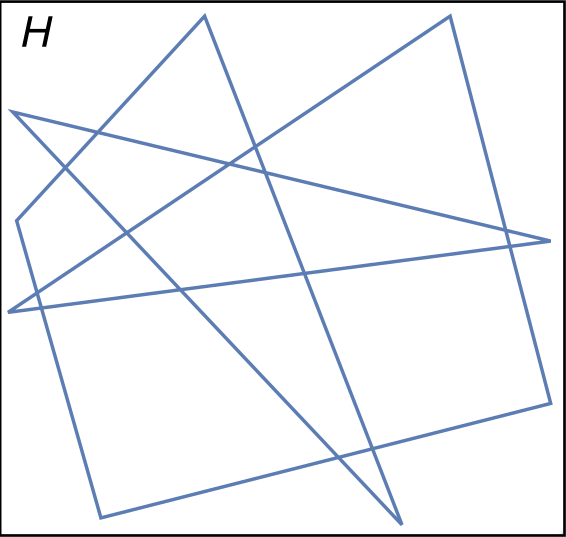
\includegraphics[width=\textwidth]{./ergodic.png}
      \caption{Ergodicity}
    \end{subfigure}
  \hfill
    \begin{subfigure}[t]{0.45\textwidth}
      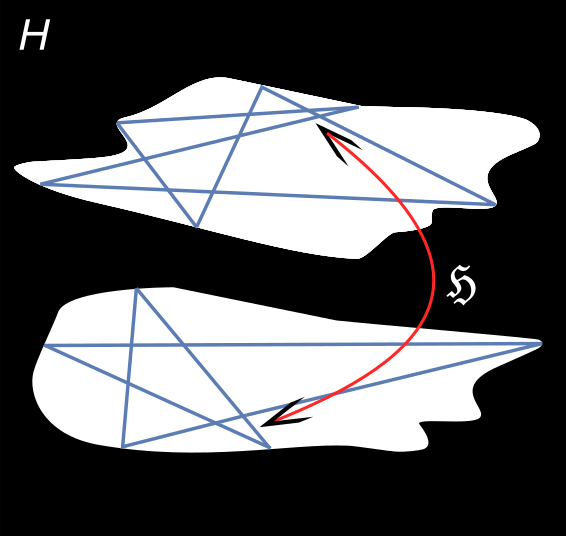
\includegraphics[width=\textwidth]{./non_ergodic.png}
      \caption{Oscillating coherences via $\mathfrak{H}$}
    \end{subfigure}
  }
  \only<3->{
    \hfill 
    \begin{subfigure}[t]{0.65\textwidth}
      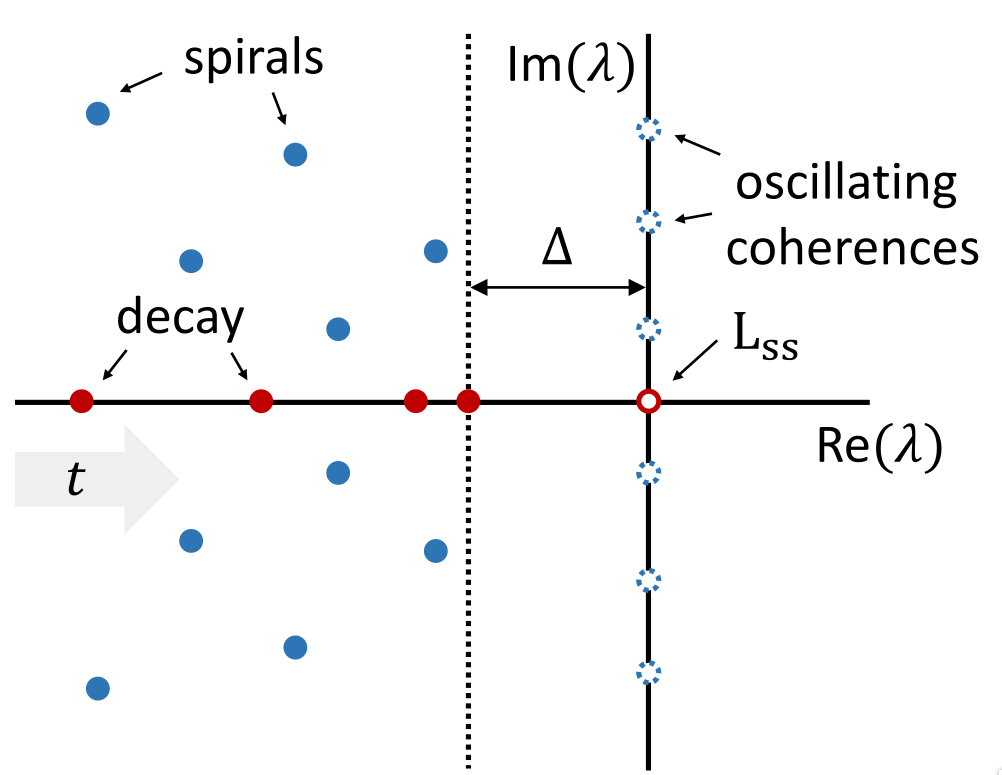
\includegraphics[width=\textwidth]{./eigenvalues_lind.png}
      \caption{Eigenvalues of $\mathcal{L}$}
    \end{subfigure}
  }
  \end{figure}

\end{column}
\end{columns}
\end{frame}

\begin{frame}{(non)-Stationarity}
  \only<1->{
  \begin{theorem}
    Let $\kett{\rho_\infty}$ - steady state, s.t. $\lan \kett{\rho_\infty} = 0$. If $\exists$ A s.t.
    $$[H,A]\rho_\infty = \lambda A \rho_\infty \qquad [L_k, A]\rho_\infty = [L_k^\dag, A]\rho_\infty  = 0$$
    Then, $$\lan (A\kett{\rho_\infty}) = i\lambda A\kett{\rho_\infty} \qquad \text{ i.e. } A\kett{\rho_\infty} \in \text{EigSp}(\lan)$$
    with $\lambda$ - purely imaginary (See oscillating coherences).
  \end{theorem}
}
\only<2->{
  Intuitively, given $\kett{\rho_\infty}$, the \textit{"symmetry"} $A$ will \textit{"induce"} the 
  non-stationary states.
}
\end{frame}

\begin{frame}{(non)-Stationarity}
  One defines
  \begin{itemize}
    \item<1-> Super-operator $\doublehat{A}$:\quad $\doublehat{A}\kett{\rho}\equiv \hat{A} \kett{\rho}$, with 
      operator $\hat{A}$ with defined properties.
    \item<2-> The state $\kett{\rho_\infty}$ as before, $\lan \kett{\rho_\infty} = 0$
    \item<3-> The eigen-operator relation for super-operators $$[\lan, \doublehat{A}] = i\lambda \doublehat{A}$$
  \end{itemize}
\end{frame}

\begin{frame}{}
    \begin{block}{Corollary}
      \only<1->{
      If there exists an operator $\hat{A}$, such that 
      $$[H,\hat{A}] = \lambda \hat{A} \qquad \text{ and } \qquad [L_k, \hat{A}]=[L_k^\dag, \hat{A}] = 0 \quad \forall k$$
    }
      \only<2->{
      Then, one can define 
      $$\kett{\rho_{nm}} = \bigl(\hat{A}\bigr)^n\, \kett{\rho_\infty}\, \bigl(\hat{A}^\dag \bigr)^m$$
    }
    \only<3->{
      Then, one has 
    $$ \boxed{\mathcal{L}\kett{\rho_{nm}} = i\lambda(n-m)\kett{\rho_{nm}}} $$
    }
  \end{block}
\begin{columns}
  \begin{column}{0.7\textwidth}
    \begin{itemize}
      \item<4-> Properties of eigenstates $\kett{\rho} \leftrightarrow \sigma(\lan)$ \\
        derived independently.
      \item<5-> Main ingredients - $\{H, L_k, \hat{A}\}$ and $\rho_\infty$
      \item<6-> Symmetry-preserving dissipations \& dark Hamiltonian
    \end{itemize}
  \end{column}
  \begin{column}{0.3\textwidth}
    \begin{figure}
      \only<4->{
        \centering
      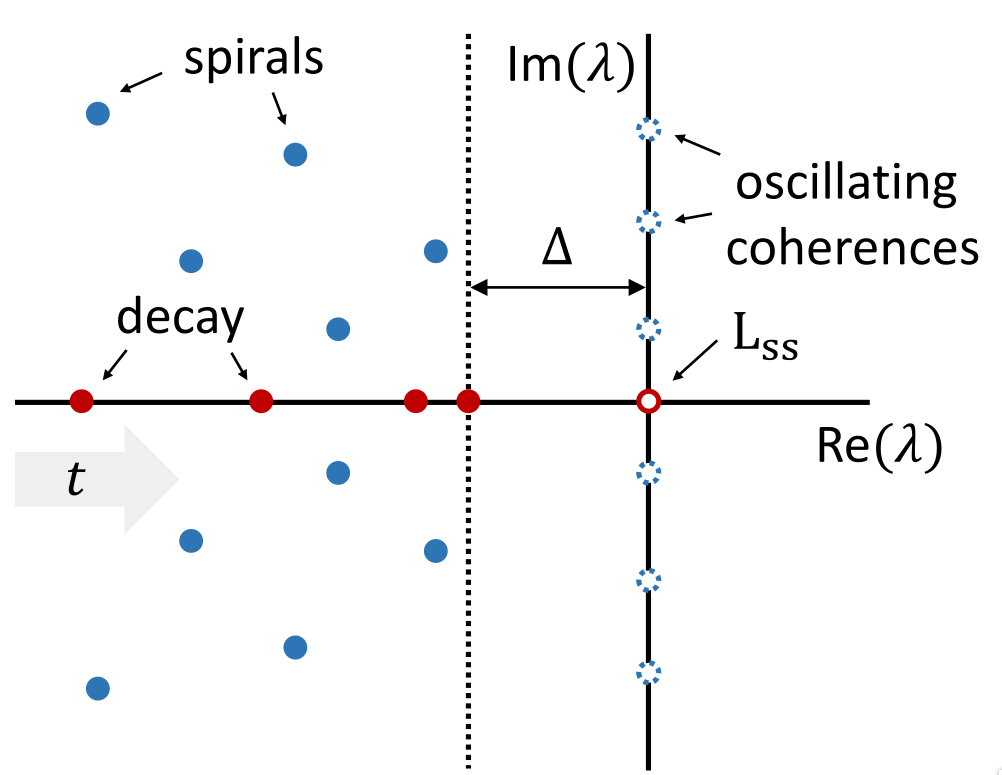
\includegraphics[width=0.9\textwidth]{./eigenvalues_lind.png}
      \caption{}
    }
    \end{figure}
  \end{column}
\end{columns}

\end{frame}

\end{document}






